Having detected the events, we still have to present them to the user in a readable format. A set of keywords may be a concise representation for the computer, but it does not offer much insight into the event itself. We aim to generate short annotations for the events, based on which the user can decide to actually inspect the event more thoroughly and read some of the documents. Consequently, we need to retrieve a number of documents relevant to each event. These documents will then be used in \autoref{chap:event-annotation} to generate summaries.

We can use each event's temporal and semantic information to query the document collection. The former is trivial -- simply select the documents published within an event's bursty period. From these document, we can then select those document which relate to the event semantically. This will prove more complicated, and we will need to employ some more information retrieval techniques to obtain the documents.

As of now, an event $e$ is described by a set of its keywords, $\kw{e}$. The goal is to convert this keyword representation to a document representation, $\doc{e}$ consisting of documents related to $e$.

\section{Event burst detection}
First, we need to detect the period when the particular event happened, so that we can retrieve the documents published around that time. This part of the algorithm again follows from \cite{event-detection}. In this paper, the period around an event's occurrence was called \textit{bursty period}. The burst detection is done in five steps.

\begin{enumerate}
	\item Construct the event trajectory from the trajectories of its keywords.
	\item Clean the event trajectory.
	\item Determine the event's periodicity.
	\item Fit a probability density function to the event trajectory.
	\item Take the region(s) with the highest density as the bursty period(s).
\end{enumerate}


\subsection{Event trajectory construction}
We first need to construct an \textit{event trajectory} out of its \textit{keyword trajectories}. We do this by computing a weighted average of the event's keyword trajectories, with weights being the keyword DPS. This ensures that less important words with slightly different time characteristic will not shift the trajectory away from the actual burst.

\begin{equation}
	\vect{\traj_{e}} = \frac{1}{\sum_{k \in \kw{e}}{\text{DPS}_{k}}} \sum_{k \in \kw{e}}{\text{DPS}_{k} \cdot \vect{\traj}_{k}}
\end{equation}

An example of such event trajectory can be found in \autoref{fig:kw-event-trajectories}.


\begin{figure}
\centering
\begin{subfigure}{.5\textwidth}
  \centering
  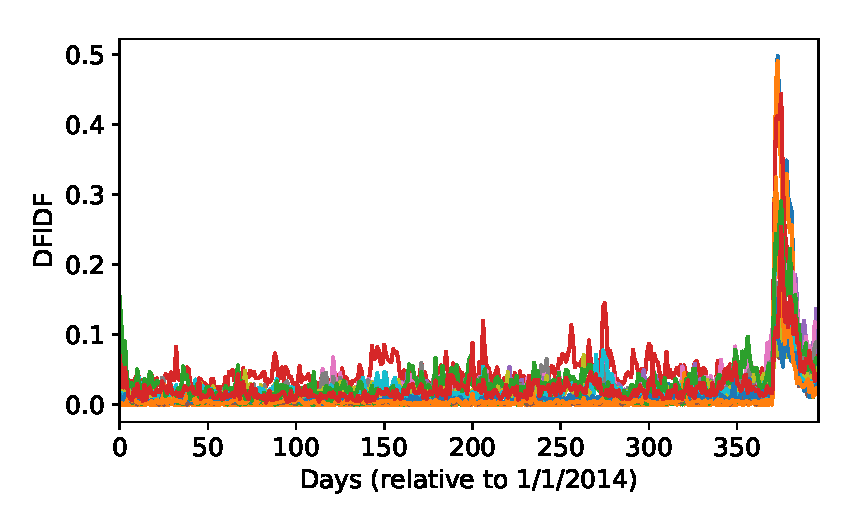
\includegraphics[width=\linewidth]{11_words_no_label}  % charlie hebdo words without labels
  \caption{Event keywords}
  \label{fig:hebdo-words}
\end{subfigure}%
\begin{subfigure}{.5\textwidth}
  \centering
  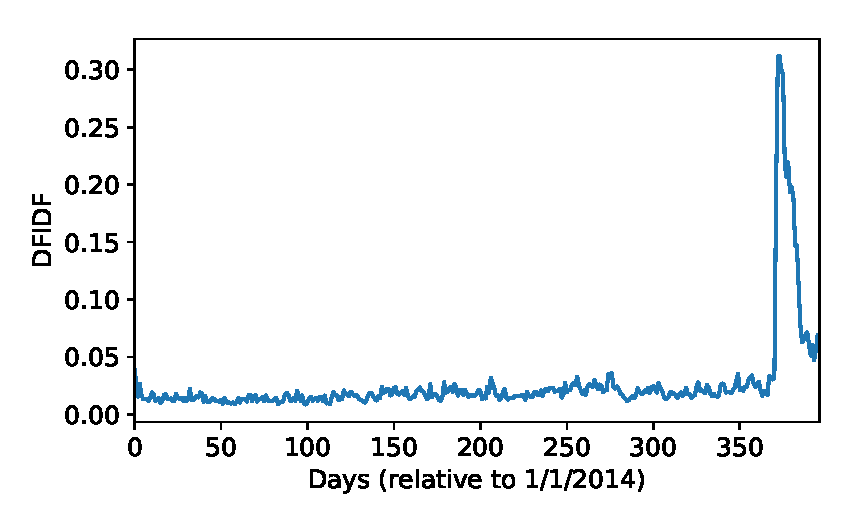
\includegraphics[width=\linewidth]{11_trajectory}  % charlie hebdo trajectory
  \caption{Event trajectory}
  \label{fig:hebdo-trajectory}
\end{subfigure}
\caption{Keywords and trajectory of the event related to Charlie Hebdo attack. The keywords are \textit{Charlie, Hebdo, Mohamed (Muhammad), Paříž (Paris), Islam, karikatura (caricature), Muslim, náboženství (religion), pařížský (Parisian), prorok (prophet), satirický (satirical), teroristický (terroristic), terorizmus (terrorism)}.}
\label{fig:kw-event-trajectories}
\end{figure}


\subsection{Trajectory filtering} \label{subsec:trajectory-filtering}

Now, a typical event (shown in \autoref{fig:vrbetice-trajectory}) usually has a number of dominant bursts corresponding to the period(s) when the event actually occurred. Additionally, there are some milder, noisy bursts due to the keywords appearing elsewhere, independently of that particular event.

We aim to fit a probability density function to the event trajectory, as in \cite{event-detection}. The noisy bursts would behave as outliers, shifting the fitted function away from the main event bursts. Once again, we apply the Burst filtering algorithm from \autoref{subsec:noise-filtering} to filter out noise, this time from the event trajectories. The cutoff value computed by the Burst filtering algorithm is shown in \autoref{fig:vrbetice-trajectory} as well.


\begin{figure}
  \centering
  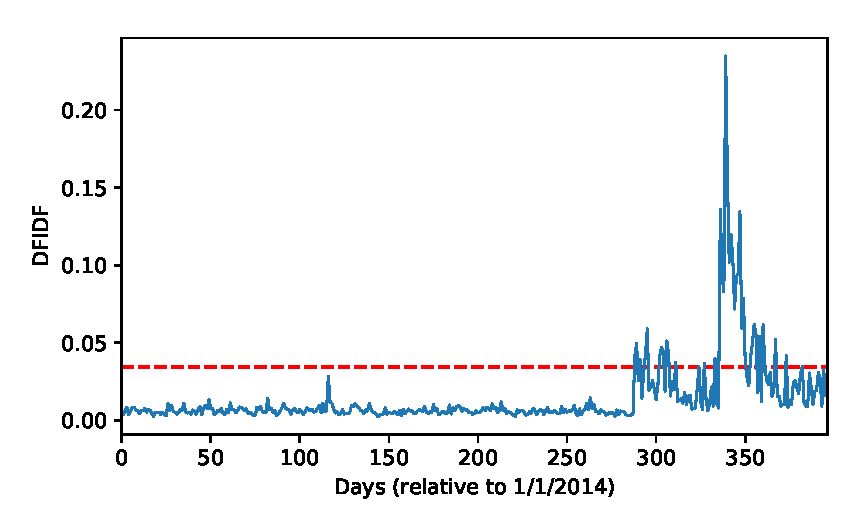
\includegraphics{41_trajectory_cutoff}  % Vrbetice trajectory with cutoff
  \caption{An event with a noisy trajectory and keywords \textit{Vrbětice, muniční (ammunition), sklad (storage)} related to the explosions of the ammunition storage in Vrbětice on October 16 and December 3, 2014 (events 38 and 47 in \autoref{app:real-events}. The dashed red line is the cutoff value computed using window length 7. The parts of the trajectory under the cutoff will be discarded.}
  \label{fig:vrbetice-trajectory}
\end{figure}


\subsection{Event periodicity}
We apply the signal processing techniques described in \autoref{chap:word-analysis} once more, this time to determine the dominant period $\domper{e}$ of each event $e$. After computing the periodogram, the dominant period is defined as the inverse of the frequency corresponding to the highest peak in the event trajectory:

\begin{equation}
	\domper{e} = \frac{\streamlen}{\argmax\limits_{k \leq \ceil{\streamlen / 2}}{\|X_{k}\|^{2}}},
\end{equation}

as the Fourier coefficient $X_{k}$ denotes the amplitude at frequency $\frac{k}{T}$. We then consider an event $e$ to be \textit{aperiodic} if it happened only once in the stream, that is if $\domper{e} > \ceil{\streamlen / 2}$. Similarly, the event is \textit{periodic} if $\domper{e} \leq \ceil{\streamlen / 2}$.

\subsection{Density fitting}
We normalize the event trajectories to have unit sums, so they can be interpreted as probability distribution over days. An element $\trajn_{e}(i)$ of the normalized trajectory $\vect{\trajn}_{e}$ can be interpreted as the probability of that event occurring on day $i$. This allows us to fit a probability density function to them. \cite{event-detection} adapted a similar approach, though only for word rather than event trajectories.

We describe aperiodic and periodic events separately, as different probability distributions must be used in case of a single burst than in case of multiple bursts.

\begin{enumerate}

\item \textbf{Aperiodic events}

An aperiodic event trajectory $\vect{\trajn}_{e}$ is modeled by a Gaussian distribution $\mathcal{N}(\mu,\,\sigma^{2})$. We fit the Gaussian function to the trajectory $\vect{\trajn}_{e}$ and estimate the parameters $\mu$ and $\sigma$. \cite{event-detection} did not mention the method they used for aperiodic trajectories. As we are fitting the density to probabilities rather than observations, Maximum Likelihood Estimate of the parameters is not applicable. We decided to use non-linear least squares, namely the Trust Region Reflective algorithm \citep{trust-region-reflective} to estimate $\mu$ and $\sigma$ bounded within the document stream period. An example of the Gaussian distribution fit to an event trajectory is shown in \autoref{fig:aperiodic-density}.

\item \textbf{Periodic events}

A periodic event trajectory $\vect{\trajn}_{e}$ is modeled using a mixture of $K = \floor{\streamlen / \domper{e}}$ Cauchy distributions (as many mixture components as there are periods), as in \cite{health-events}:

\begin{equation*}
	f(x) = \sum_{k = 1}^{K}{\alpha_{k} \frac{1}{\pi} \left( \frac{\gamma_{k}}{\left( x - \mu_{k} \right)^{2} + \gamma_{k}^{2}} \right)}
\end{equation*}

The mixing parameters $\alpha_{k} \geq 0,\ \sum_{k = 1}^{K}{\alpha_{k}} = 1$, location parameters $\mu_{k}$ and scale parameters $\gamma_{k}$ are estimated using the EM algorithm.

The Cauchy distribution has a narrower peak and thicker tails than the Gaussian distribution, which models the periodic bursts more closely. The individual bursts of a periodic event tend to be quite short, but even between two consecutive bursts, the frequency remains at a non-negligible level, which makes the Cauchy distribution a somewhat better choice. \autoref{fig:periodic-density} shows an example of such fit.

\end{enumerate}

\begin{figure}
  \centering
  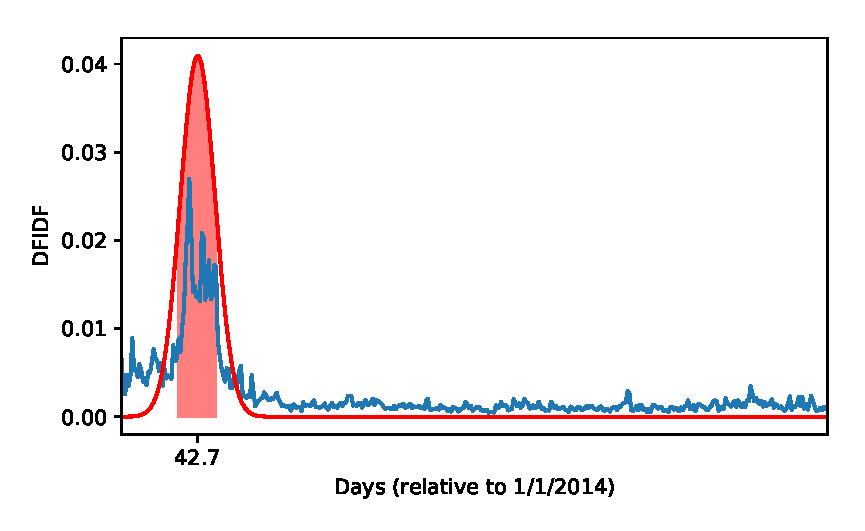
\includegraphics{39_density_fit}  % aperiodic event (olympiada)
  \caption{An aperiodic event consisting of the keywords \textit{Sochi, ZOH (Winter Olympic Games), olympijský (olympic), olympiáda (olympiad)}. The Gaussian function modeling the trajectory and the event bursty period are shown in red.}
  \label{fig:aperiodic-density}
\end{figure}


\begin{figure}
  \centering
  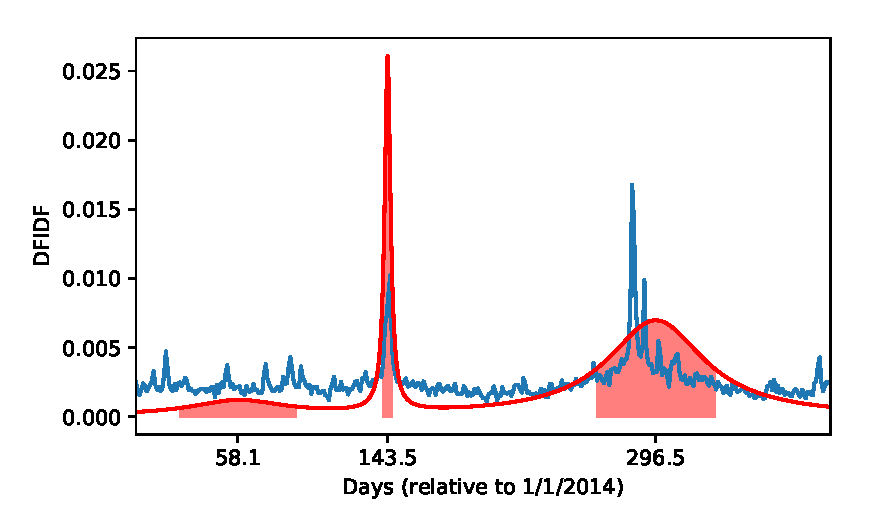
\includegraphics{63_density_fit}  % periodic event
  \caption{A periodic event with keywords \textit{volba (election), volební (electoral), volič (voter)} and a period of 132 days. The event is modeled by a mixture of $\floor{396/132} = 3$ Cauchy distributions. Each of the event's bursty periods is highlighted.}
  \label{fig:periodic-density}
\end{figure}


\subsection{Burst detection}
Using the fitted probability density functions, we define the bursty period(s) as the regions with the highest density. The bursty period of an aperiodic event $e$ is now defined as $\bursts{e} = \left\{ \interval{\mu - \sigma}{\mu + \sigma} \right\}$. For a periodic event, there are $K = \floor{\streamlen / \domper{e}}$ bursty periods defined as $\bursts{e} = \left\{ \interval{\mu_{k} - \gamma_{k}}{\mu_{k} + \gamma_{k}} \mid k = 1, \dots, K \right\}$. The burst of an aperiodic event is highlighted in \autoref{fig:aperiodic-density}, while a periodic event's bursts are shown in \autoref{fig:periodic-density}.


\section{Document retrieval}
We only describe the process for aperiodic events. The method is similar for periodic events, except applied on each burst individually.

We need to measure the relevance of individual documents published within an event's bursty period to the event. The only measure of semantics for an event we have is the event's keyword set $\kw{e}$. If we interpret $\kw{e}$ as a keyword query for the document collection, we arrive at the classical task of Information Retrieval. That is, to rate the documents in a given corpus by their relevance to the query \citep{information-retrieval}.

In the original method by \cite{event-detection}, the task was simple due to the cost function used. The only measure of semantic similarity was the degree of document overlap between all words in $\kw{e}$. If two words had no document overlap, they would not get assigned in the same event. That way, there was always at least one document in which all of the event's keywords appeared. It was a simple matter to compute the intersection of all documents containing either keyword within the bursty period. This is not the case in our method, and we will need to measure the document relevance in a more sophisticated way.

There are a few approaches we could take, such as project all documents and queries to a TFIDF (Term Frequency-Inverse Document Frequency) space \citep{information-retrieval} and sort the documents by their cosine similarity to the query. This simple approach does not go beyond a trivial keyword occurrence comparison, though after applying some weighting scheme. We could enrich it using Latent Semantic Indexing \citep{lsi} to also take the document topics into account. This would require us to compute yet another model to be used for this part only, which would be computationally and memory-intensive.

Instead, we decided to further utilize the Word2Vec model and use the recently introduced Word Mover's Distance \citep{wmd}, which is an application of the better known measure of Earth Mover's Distance \citep{emd} to word embeddings.

The Word Mover's Distance (WMD) measures the similarity of two documents as the minimum distance the word vectors of one document need to ``travel'' to reach the word vectors of the second document. Since more similar words are embedded close to each other \citep{linguistic-regularities}, the farther apart the words lie, the less similar they are semantically. The formal definition of the WMD is rather lengthy, so we refer the reader to the original paper \citep{wmd} for the full derivation.

The WMD discards word order, which makes it suitable for our keyword queries. As the authors note, it achieves best results for short documents, in part due to the method being computationally expensive for larger pieces of text. Therefore, we apply the WMD to document headlines only.

In Information Retrieval, it is more traditional to work with document similarity rather than distance. In the Gensim framework \citep{gensim} which implements the WMD, the similarity is defined as

\begin{equation}
	\wmdsim{d_{i}}{d_{j}} = \frac{1}{1 + \wmd{d_{i}}{d_{j}}}
\end{equation}

which is 1 if $\wmd{d_{i}}{d_{j}} = 0$ and goes to 0 as $\wmd{d_{i}}{d_{j}} \to \infty$.

We now describe the algorithm to compute the document representation of an event.

\begin{algorithm}[H]
\begin{algorithmic}[1]
\caption{Document representation of an aperiodic event}
\label{alg:doc-retrieval}
\Input $\text{Event}\ e,\ \mathit{burst} \in \bursts{e},\ \text{number of documents}\ n,\ \text{document stream}\ D$

\State $\mathit{burst\_docs} = \emptyset$

\ForEach{$\mathit{doc} \in D$}
	\If{$\mathit{doc.publication\_date} \in \mathit{burst}$}
		\State $\text{Compute}\ \wmdsim{\kw{e}}{\mathit{doc.headline}}$
		\State $\mathit{burst\_docs} = \mathit{burst\_docs} \cup \mathit{doc}$
	\EndIf
\EndFor

\State $\text{Sort}\ \mathit{burst\_docs}\ \text{by the computed}\ \text{Sim}_{\text{WMD}} \ \text{in descending order}$
\Output $\text{first}\ n\ \text{elements of}\ \mathit{burst\_docs}$
\end{algorithmic}
\end{algorithm}

The set of event documents $\doc{e}$ is then a union of the outputs of Algorithm \ref{alg:doc-retrieval} over all bursts in $\bursts{e}$.

In our experiments, we chose the number of documents $n$ as the square root of total number of documents within the particular event burst.